\section{Specification}\label{sec:spec}
% section specification

The requirements specification identifies the target users of the Colladoc Smart Search and goes over the product use cases. The requirements, use cases and queries are prioritized in two categories:

\begin{itemize}
\item  Essential - describe functionality that is fundamental to the project and will be implemented during  the development stage.

\item  Non-Essential - describe functionality that would be beneficial to the project but is not guaranteed to be delivered.
\end{itemize}

\subsection{Target Users}

[u1] Developer - a person with working knowledge in Scala. Sometimes he searches for packages, classes, objects etc. The developer searches for something specific.

[u2] Technical Writer - a person responsible for writing documentation. He needs a quick 
overview of missing or updated documentation. He needs to limit searches to the packages and classes that he is working on.

[u3] Beginner - a person learning the Scala language or starting on a Scala-based project. He may not be familiar with Scala syntax and needs helpful search results from general queries.

\subsection{Functional Requirements}

\subsubsection{Essential Functional Requirements}
\indent [c1] When the user enters a search query, the search results page should displays all entities that match the query. 
We have implemented all essential queries that were planned \emph{\color{red}see example queries}.

[c2] When the user is on the search results page, clicking on the entity name (1) toggles its details (2).
We have implemented this functionality.

\begin{figure}[h!t]
\begin{center}
\leavevmode
\fbox{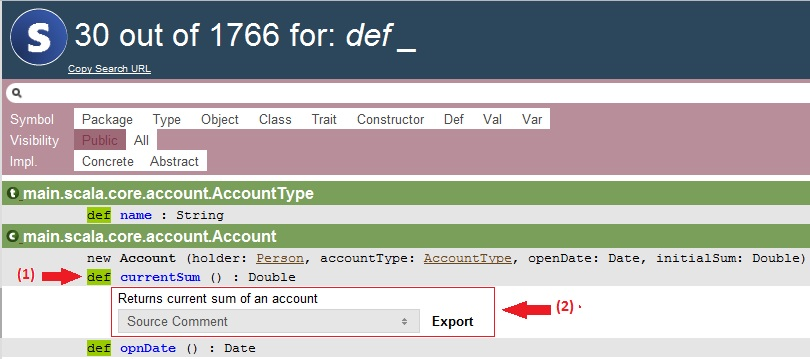
\includegraphics[width=0.9\textwidth]{c2}}
\end{center}
\caption{Toggle User Details}
\label{fig:toggle_user_details}
\end{figure}


[c3] When the user does not enter anything, search is not triggered.
We have implemented this functionality.

[c4] The search result page support filtering of the results. Filtering can be done either by entity type using predefined filters (2) or by entity name (1) . 
We have implemented this functionality.
\begin{figure}[h!t]
\begin{center}
\leavevmode
\fbox{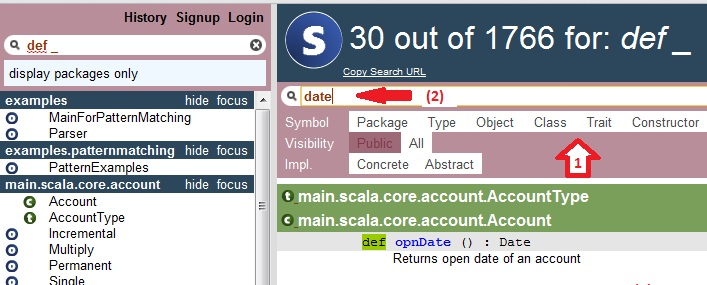
\includegraphics[width=0.9\textwidth]{c4}}
\end{center}
\caption{Filter Results}
\label{fig:filter_results}
\end{figure}

[c5] When entity comment is updated, searching the changed documentation should contain the updated entities.
We have implemented this functionality.

\textbf{Essential Query Examples}

Table~\ref{essential_query_examples} contains examples of the essential query language constructs. 
\begin{table}[htbp]
\begin{center}
\begin{tabular}{|p{1.4in}|p{0.7in}|p{1.8in}|p{0.4in}|} \hline 
\textbf{User Query/Search} & \textbf{Syntax} & \textbf{Results Produced} & Status  \\ \hline 
[q1] Any text ``Foo''. & Foo & - Comments that contain text ``Foo''\newline - All entities (types/packages/methods) with names containing the text Fooe.g. class FooBar, trait MyFooTrait & done \\ \hline 
[q2] Text ``Foo'' exactly. & ``Foo'' & - Comments that contain ``Foo'' exactly\newline - Entities named exactly ``Foo'' & done \\ \hline 
[q3] Text ``Foo'' in comments. & // Foo & Comments that contain text ``Foo''. & done \\ \hline 
[q4] Classes\textbackslash objects\textbackslash \textbf{ }
traits\textbackslash packages named ``Foo''. & class Foo; object Foo; trait Foo; package Foo & Entities named ``Foo'' exactly. & done \\ \hline 
[q5] Classes\textbackslash objects\textbackslash \textbf{ } traits\textbackslash packages whose names end with ``Foo'' & class \_Foo; object \_Footrait \_Foo; package \_Foo & Entities with names ending with ``Foo''.\newline e.g. Foo, MyFoo & done \\ \hline 
[q6] Classes that extend class ``BaseFoo'' & extends BaseFoo & All classes that derive from ``BaseFoo''.\newline e.g. DerivedFoo & done \\ \hline 
[q7] Classes that implement trait ``FooTrait'' & with FooTrait & All classes that implement the trait ``FooTrait''. & done \\ \hline 
[q8] Methods named ``bar'' & def bar & All methods (any number of parameters and any return type) that are named ``bar'' & done \\ \hline 
[q9] Methods that return Int & def \_ : Int & All methods that return Int & done \\ \hline 
[q10] Methods that have two parameters, an Int and a String, and return Int & def \_(Int, String): Int & All methods that take an Int and a String and return Int. e.g. bar(i: Int, s: String) : Int\newline \newline This will also return equivalent curried functions e.g. bar(Int)(String) & done \\ \hline 
[q11] Method that takes an Int parameter, followed by zero or more parameters & def \_(Int, *) & All methods that take an Int and zero or more parameters & done \\ \hline 
[q12]  Values or variables called ``name'' & val name:String\newline var name:String & All member values or variables that are named ``name'' and are of type String. The results are ordered by val / var depending on the query. & partial \\ \hline 
\end{tabular}
\caption{Essential Query Examples}
\label{essential_query_examples}
\end{center}
\end{table}

\subsubsection{Non Essential Functional Requirements} 
\indent \indent [c6] Technical Writer searches for the entities in a package. Then he filters the results to entities with no documentation by selecting an option on the page. We have not implemented this requirement due to time constraints, but the system can be easily extended to support it.

[c7] The user searches for the entities in a package. If no result is found, a help page is displayed. The help page contains sample queries that (1) as well as option for searching that query input in Google (2).
We have implemented this functionality. Additionally, we have provided a Syntax Reference page that provides query examples for the supported syntax.

\begin{figure}[h!t]
\begin{center}
\leavevmode
\fbox{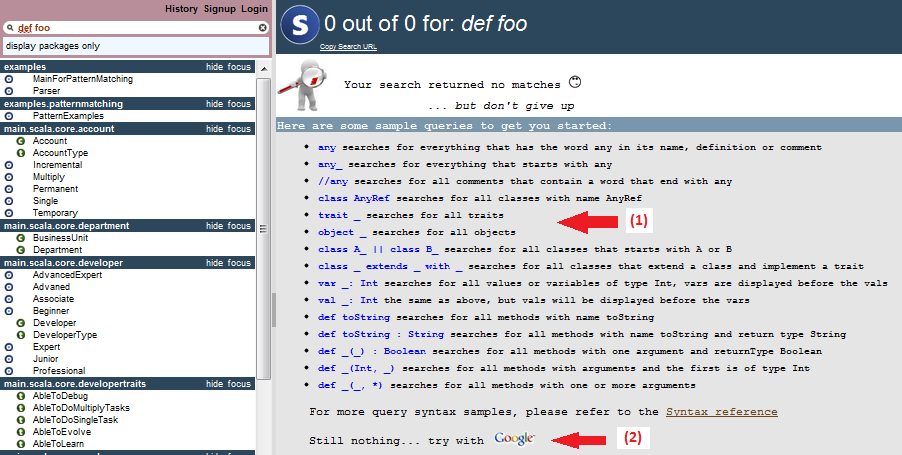
\includegraphics[width=0.9\textwidth]{c7}}
\end{center}
\caption{Filter Results}
\label{fig:filter_results}
\end{figure}

[c8] The user searches for an entity. If there is only one search match, the result will be the documentation page of the given entity.
We have not implemented this requirement due to time constraints.

[c9] The user browses the search results. He wants to see only one type of entity. He chooses this by clicking an option in the results filter. 
We have implemented this functionality.

[c10] The Developer wants to see where a class is used in the API. He searches for the exact name of the class. The search returns all the API visible usages of the class. As a result of discussion with our supervisors, we decided that this requirement does not provide any benefits to the current project and is not related to our final goal. Therefore, this functionality was not implemented.

[c11] A user searches for the entities in a package. Then he filters the results to entities that contain code snippets in their comments.
After discussion with our supervisors, we set low priority for this requirement. We do not see this feature providing great benefit to the user. There are better ways to look for code snippets: blogs, articles and so on. Moreover,  we could not find any example of code in the comments of the codebases we looked at. We have not implemented this functionality.

We have managed to extend the query syntax so it supports most of the initially specified non-essential queries. 

The syntax that is not currently supported is [q13] and [q20]. [q13] was not implemented because of the large development effort required. Additionally, omitting this query does not limit what the user can search for. [q20] was not implemented due to time constraints. 

We recognised that our initial query syntax specifications did not support some important queries. We realised that if we omitted these queries, it would restrict the users ability to search for some language constructs. Therefore, we have added two more search features to the syntax: search for tuples [q21] and search for entities with reserved names [q22]. This is supported by the language and is commonly used in many Scala libraries. 

Additionally, we changed the syntax of query [q18] in order to comply with the Scala syntax. Also [q12] is partially imported - the syntax is supported, but due to time constraint we have not implemented ordering based on whether the user search for val or var.

\textbf{Non-Essential Query Examples}

Table~\ref{non_essential_query_examples} contains examples of the essential query language constructs. 
\begin{table}[htbp]
\begin{center}
\begin{tabular}{|p{1.4in}|p{1.2in}|p{1.3in}|p{0.5in}|} \hline 
\textbf{  User Query/Search Syntax}\newline \textbf{} & \textbf{Syntax } & \textbf{Results Produced} & \textbf{Status} \\ \hline 
[q13] Search using logical AND. e.g. search for classes named ``Foo'' and classes that contain a method ``bar''. & class Foo AND def barclass Foo \&\& def bar & All classes named Foo that contain a method bar & not done \\ \hline 
[q14] Search using logical OR.\newline e.g. search for methods named ``add'' or methods named ``sub'' & def add OR def sub\newline def add \textbar \textbar  def sub & All methods named ``add'' or methods named ``sub''. & done \\ \hline 
[q15] Search using the NOT operator. e.g. search for classes that end with text ``Foo'', but exclude classes named ``BaseFoo'' from the results & class \_Foo not class BaseFoo\newline class \_Foo !class BaseFoo & All classes that end with ``Foo'' but not class ``BaseFoo'' & done \\ \hline 
[q16] Search using query grouping. e.g. search for classes named ``Bar'' or for classes with names ending in ``Foo'' but not ``BaseFoo'' & class Bar OR (class \_Foo NOT class BaseFoo) & All classes named Bar in addition to classes that end with ``Foo'' but not class ``BaseFoo'' & done \\ \hline 
[q17] Search for method that takes a function as a parameter. & def \_(Int =$>$ String) & All methods that take one parameter which is a function with signature Int =$>$ String & done \\ \hline 
[q18] Search for all methods with two parameters, an Int and a String, and return Int & Int =$>$ String =$>$ Int\newline (Int, String) =$>$ Int & All methods that take an Int and a String and return Int.\newline e.g. bar(i: Int, s: String) : Int & modified \\ \hline 
[q19] Search for a generic class with one parameter & class \_[A] & All classes with one generic parameter & done \\ \hline 
[q20] Search for a generic method called ``foo'' with two generic parameters. & def foo[A,B](A, B, Int) & Returns all methods called foo with two generic parameters and the respective argument types. & not done \\ \hline 
[q21] Search for Tuples & def \_:(A,B) & Returns all methods that return a two-element tuple with of types A and B & done\newline (new) \\ \hline 
[q22] Search for keywords & def `def` & Returns all methods named ``def'' & done\newline (new) \\ \hline 
\end{tabular}
\caption{Non-Essential Query Examples}
\label{non_essential_query_examples}
\end{center}
\end{table}

\subsection{Non-Functional Requirements}

\subsubsection{Essential Non-Functional Requirements}


[n1] The search results should appear in less than 5 seconds. 
We have achieved this requirement. With the largest codebase we have tried, the results appeared in less than two seconds. For more details, see Final Product - Performance section.

[n2] The source code of Colladoc Smart Search will contain unit tests for most of the newly added classes.
We have achieved \emph{\color{red}92} \% code coverage.For more details, see \emph{\color{red} Final Product - Testing}.
[n3]The source code will follow the coding style and formatting of the existing Colladoc code.
This requirement has been achieved. We have created Coding Style document \cite{coding-style} and have adhered to it throughout development. 

\subsubsection{Non Essential Non-Functional Requirements}

[n4] End-to-end integration tests for the essential search functionality will be created.
This requirement has been achieved. For more details, see Final Product - Testing.
[n5] The results should be displayed immediately in the results page. The user should not wait for all of the results to be fetched if they are more than 5 entities.
This requirement has been achieved. \emph{\color{red} See Design- Infinite scrolling section}
